% Drawing 144/07-7 -- folder 144, batch 07, archive page 133 (PDF page 134).
% Transcription: au crayon, très pâle, une esquisse d'un cube plus grand : $\mathcal{M}^!(0)\to\mathcal{M}^!_\Pi[0]$, $\mathcal{M}^!$, $\mu_\tau$, $D^\Pi_0$, $\mathcal{M}^!_{\mathfrak{S}}[0]$, $\mathcal{M}$, $1$, $L^\Pi_0$, $D^{\mathfrak{S}}_0$, $\Pi$, $\mathfrak{S}$, $L^{\mathfrak{S}}_0$, $\mathfrak{S}^+$, et plus bas $\Pi' = \mathfrak{S}^!$, $\Pi = \mathfrak{S}^{!+}$, $\mathfrak{S}^+$, $\mathcal{M}^{!+}$, $\mathcal{M}^+$ — premier état du cube de la p.~135.
% Kind: pale pencil sketch of a larger cube (first state of p. 135). Method 2 (schematic redraw from the facsimile). Status: partial.
% Notes: Very pale pencil, re-read on a contrast-enhanced tight crop; everything drawn as pencil. Upper right: the rows M^!(0) -> M^!_Pi[0] -- M^!; mu_tau -- D^Pi_0 -- M^!_S[0] -- Pi' -- M; 1 -- L^Pi_0 -- D^S_0 -- Pi -- S; L^S_0 -- S^+, with the short verticals between rows, the diagonals D^Pi_0 -- D^S_0, L^Pi_0 -2- L^S_0, M^!_Pi[0] -- M^!_S[0], M^! -- M and Pi -- S^+, each stroke where it is on the page between the labels. Lower left: Pi' = S^! and Pi = S^{!+} with their horizontal strokes, S^+, M^{!+}, M^+ and the strokes joining them. Labels \small. Still differs from the facsimile: the strokes are too faint to tell arrow from line (only M^!(0) -> M^!_Pi[0] shows a head) and some short ones may be missed; the label read Pi' in the second row is not in the transcription's list (a reading); a few faint marks left of the lower part are left out. Redrawn 2026-11-09 (issue 128): to check again.
% Coordinates: 1 unit = 1 mm = 1/100 of the crop width (bbox in page fractions: [0.28, 0.65, 0.92, 0.86]).
% Redrawn by Claude (claude-opus-5-5), issue #73, 2026-11-09; not checked by a human; not compiled (no TeX in the session).
% Rights: reproduces part of the work -- behind RENDER_TRANSCRIPTS, never published by itself.
\documentclass[tikz,border=3pt]{standalone}
\usepackage{amsmath,amssymb}
\usetikzlibrary{patterns,arrows.meta}
\tikzset{pencil/.style={black!45}, struck/.style={black!35}, mark/.style={circle,draw,inner sep=1.3pt}, pt/.style={circle,fill,inner sep=0.9pt}, opt/.style={circle,draw,fill=white,inner sep=1.1pt}}
\begin{document}
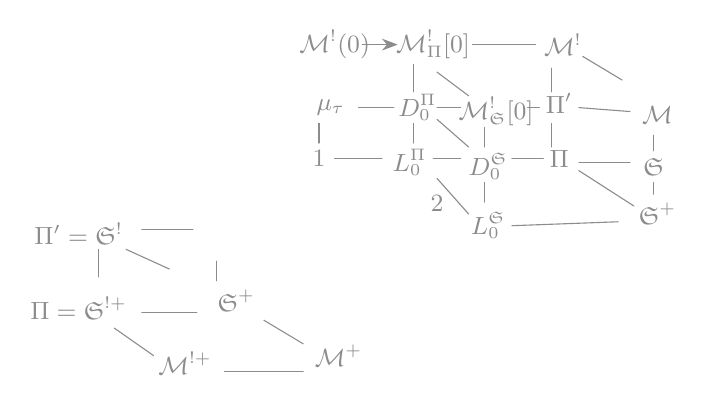
\begin{tikzpicture}[x=1mm,y=1mm,line cap=round,line join=round,font=\scriptsize]
\draw[pencil,-{Stealth[length=2mm]}] (47.5,-3.8) -- (52,-3.8);
\draw[pencil] (61.5,-3.8) -- (69.5,-3.8);
\draw[pencil] (75.5,-5.3) -- (80.5,-8.3);
\draw[pencil] (47,-11.8) -- (51.5,-11.8);
\draw[pencil] (57,-11.8) -- (60,-11.8);
\draw[pencil] (68.5,-11.8) -- (70,-11.8);
\draw[pencil] (75,-11.8) -- (81.5,-12.3);
\draw[pencil] (44,-18.3) -- (50,-18.3);
\draw[pencil] (56.5,-18.3) -- (60,-18.3);
\draw[pencil] (66.5,-18.3) -- (70.5,-18.3);
\draw[pencil] (75,-18.8) -- (81.5,-18.8);
\draw[pencil] (66.5,-26.8) -- (80,-26.3);
\draw[pencil] (54,-6.3) -- (54,-9.8);
\draw[pencil] (54,-13.8) -- (54,-16.3);
\draw[pencil] (63,-14.3) -- (63,-16.8);
\draw[pencil] (63,-21.3) -- (63,-23.8);
\draw[pencil] (71.5,-6.8) -- (71.5,-9.8);
\draw[pencil] (71.5,-13.8) -- (71.5,-16.8);
\draw[pencil] (84.5,-15.3) -- (84.5,-17.3);
\draw[pencil] (84.5,-21.3) -- (84.5,-22.8);
\draw[pencil] (42,-13.8) -- (42,-16.3);
\draw[pencil] (57,-13.3) -- (61,-16.8);
\draw[pencil] (57,-20.8) -- (61,-25.3);
\draw[pencil] (57,-7.3) -- (61,-10.3);
\draw[pencil] (75,-19.8) -- (82,-24.3);
\node[inner sep=1pt,pencil] at (44,-3.8) {\small $\mathcal{M}^!(0)$};
\node[inner sep=1pt,pencil] at (56.5,-3.8) {\small $\mathcal{M}^!_\Pi[0]$};
\node[inner sep=1pt,pencil] at (73,-3.8) {\small $\mathcal{M}^!$};
\node[inner sep=1pt,pencil] at (43.5,-11.8) {\small $\mu_\tau$};
\node[inner sep=1pt,pencil] at (54.5,-11.8) {\small $D^\Pi_0$};
\node[inner sep=1pt,pencil] at (64.5,-12.3) {\small $\mathcal{M}^!_{\mathfrak{S}}[0]$};
\node[inner sep=1pt,pencil] at (72.5,-11.3) {\small $\Pi'$};
\node[inner sep=1pt,pencil] at (85,-12.8) {\small $\mathcal{M}$};
\node[inner sep=1pt,pencil] at (42,-18.3) {\small $1$};
\node[inner sep=1pt,pencil] at (53.5,-18.8) {\small $L^\Pi_0$};
\node[inner sep=1pt,pencil] at (63.5,-19.3) {\small $D^{\mathfrak{S}}_0$};
\node[inner sep=1pt,pencil] at (72.5,-18.3) {\small $\Pi$};
\node[inner sep=1pt,pencil] at (84.5,-19.3) {\small $\mathfrak{S}$};
\node[inner sep=1pt,pencil] at (63.5,-26.8) {\small $L^{\mathfrak{S}}_0$};
\node[inner sep=1pt,pencil] at (85,-25.3) {\small $\mathfrak{S}^+$};
\node[inner sep=1pt,pencil] at (57,-24) {\small $2$};
\draw[pencil] (19.5,-27.3) -- (26,-27.3);
\draw[pencil] (19.5,-37.8) -- (26.5,-37.8);
\draw[pencil] (17.5,-29.8) -- (23,-32.3);
\draw[pencil] (16,-39.8) -- (21,-43.3);
\draw[pencil] (35,-38.8) -- (40,-41.8);
\draw[pencil] (30,-45.3) -- (40,-45.3);
\draw[pencil] (14,-29.8) -- (14,-33.3);
\draw[pencil] (29,-31.3) -- (29,-33.8);
\node[inner sep=1pt,pencil] at (11.5,-27.8) {\small $\Pi'=\mathfrak{S}^!$};
\node[inner sep=1pt,pencil] at (11.5,-37.3) {\small $\Pi=\mathfrak{S}^{!+}$};
\node[inner sep=1pt,pencil] at (31.5,-36.3) {\small $\mathfrak{S}^+$};
\node[inner sep=1pt,pencil] at (25,-44.3) {\small $\mathcal{M}^{!+}$};
\node[inner sep=1pt,pencil] at (44.5,-43.3) {\small $\mathcal{M}^+$};
\end{tikzpicture}
\end{document}
